\chapter{Background Theory}

Development of a pneumatic pressure driven flow system for use in microfluidic research requires a firm grasp on the transition from 'macro' fluidics to microfluidics. The system operates across a great range of scales drawing and compressing air from a room of several cubic meters that is subsequently used to provide flow in channels of only a few micrometers. Following the flow path of the system - compressed air is filtered and directed via large diameter $(~5mm)$ tubing to reagent columns of large diameter $(~2cm)$, where the compressed air acts on the reagent to produce flow through smaller tubing $(<1mm)$ before finally transitioning into the microfluidic device where channel dimensions are on the order of magnitude of micrometers. This range of scale is illustrated in Figure \vref{fig:systemScale}

\begin{figure}[h]
\centering 
\includegraphics[width=0.60\columnwidth]{systemScale.PNG} 
\caption[System Scales]{Illustration of the scales involved in the system.} % The text in the square bracket is the caption for the list of figures while the text in the curly brackets is the figure caption
\label{fig:systemScale} 
\end{figure}

\clearpage

The importance of forces that act on fluids therefore dramatically changes from the macro- to the microscale. With downscaling, the buoyancy, gravitational and inertial forces are less and less important and viscous and interfacial forces become more and more predominant.\cite{Shui2007}


\section{Droplet microfluidics Overview}
Phase is a distinct state of matter in a system; matter that is identical in chemical composition and physical state and separated from other material by the phase boundary. Multiphase fluids are those in which there exist at least two different fluids in a system with different chemical composi- tions ? liquid/liquid, or with different physical states ? gas/ liquid.\cite{Shui2007}. Here we neglect consideration of gas-liquid two phase systems. 


\cite{Yang2010,Shui2007a,Zhao2011}


The study of fluid dynamics requires the analysis of individual fluid forces (such as gravity, inertial, viscous, and interfacial forces) and an understanding of how these forces combine to define fluid behavior. In order to understand the transition from large dimension $(>1mm)$ to small dimension $(<1mm)$ systems it may be useful to understand how these forces relate to system dimensions by the way of scaling laws. Some fluid forces such as inertial forces and gravity forces are dependent on the \emph{volume} of fluid involved. Other fluid forces are intrinsically defined by the \emph{surface area} of the fluids such as viscous forces and interfacial forces. More broadly speaking each of various fluid forces may be dependent on the different orders of characteristic length, $l$. For example, inertial force is dependent on density, $\rho$, which may be expressed as mass per volume or mass per $l^3$, as shown in Equation \vref{eq:inertia}. Similarly, interfacial tension is often defined as the partial differential of the Gibb's free energy over area, where the area term may be expressed in terms of $l^2$, shown in Equation \vref{eq:interfacial}.


\begin{equation}
i = \rho \nu^2 = \frac{m}{V}\nu^2 = \frac{m}{(l^3)}\nu^2 
\label{eq:inertia}
\end{equation}

%Probably wont use this eqn:
%\begin{equation}
%P = \rho g h = \frac{m}{V}g h
%\label{eq:pressure}
%\end{equation}

\begin{equation}
\gamma = \frac{\partial G}{\partial A} = \frac{\partial G}{\partial (l^2)}
\label{eq:interfacial}
\end{equation}


Consider the relative effect these individual forces have on the overall fluid behavior in which the volume dependent forces have an $l^3$ term and the surface forces have a $l^2$ term, as shown in Equation \vref{eq:scalingLaw} \cite{bruus2008}

\begin{equation}
\frac{Surface Forces}{Volume Forces} \propto \frac{l^2}{l^3} = l^{-1} \lim_{l \to 0}  \rightarrow \infty
\label{eq:scalingLaw}
\end{equation}

From this comes the realization that as systems are miniaturized towards a theoretical zero-dimension the surface forces begin play an exponentially larger effect relative to the volume forces.

\paragraph{Navier-Stokes} Early attempts at approximating fluid flow by Bernoulli and his pupil Euler completely neglected the viscosity term (an aforementioned surface force) in their mathematical expressions. In systems of small dimensions the viscosity effects are dominant and these approximations are inadequate. The Navier-Stokes expression accommodates viscous forces and is essentially a statement of force balance between inertial, pressure and viscous forces, shown in Equation . In most microfluidic systems the inertial forces are small enough that they may be neglected and the expression reduces to the statement that the net pressure forces are equal to the negative net viscous forces \cite{Vyawahare2014}.

\begin{equation}
\rho \Bigg(\frac {\partial \nu}{\partial t} + \nu \cdot \nabla \nu \Bigg) = - \nabla P+ f +\eta \nabla^2 \nu + \nabla \sigma
\label{eq:navierStokes}
\end{equation}

\begin{equation}
\frac {\partial \nu}{\partial t} + \nabla \cdot  ( \rho \nu) = 0
\label{eq:navierCOM}
\end{equation}

\begin{equation}
\rho \frac {\partial \nu}{\partial t} = - \nabla P+ f +\eta \nabla^2 \nu + \nabla \sigma
\label{eq:navierCOM}
\end{equation}

\^ above equations from \cite{Shui2007}

\paragraph{Dimensionless Groups} In many cases fluid flow at the microscale can be best categorized by comparing \emph{dimensionless groups} driven by fluid parameters such as viscosity, velocity, density and system geometry, as is the case of the dimensionless group known as Reynold's Number \emph{(Re)} shown in Equation ~\vref{eq:reynolds} . Regardless of the specific fluid or geometric parameters, systems with similar \emph{Re}  numbers general behave similarly - making it  powerful tool in characterization of a microfluidic system. The \emph{Re} value can be described in real world terms as a relation between the inertial forces and viscosity forces at play in a system. At the microscale viscous forces are dominant over inertial forces thus the \emph{Re} value is typically very low, indicating flow is laminar \cite{Kleinstreuer2013}.

\begin{equation}
Re =\frac {\rho \nu L}{\mu}
\label{eq:reynolds}
\end{equation}

Where $\rho$ is fluid density, $\nu$ is fluid velocity, $L$ is characteristic length, and $\mu$ is fluid viscosity. The \emph{Re} value dictates whether the system will be within the laminar or turbulent regime. \emph{Re} values tend to be small $(< 1)$ for microfluidic systems because the spatial scales, and therefore characteristic length, are small while fluid viscosity is constant relative to larger-scale systems \cite{D??azNafr??a2013}. As the majority of microfluidic systems feature small \emph{Re} numbers inertial forces are overwhelmed by interfacial forces in resulting in laminar flow and the dimensionless group becomes less valuable in the differentiation and categorization of different systems\cite{Shui2007}.

The Capillary number \emph{(Ca)} is a dimensionless group that compares the relative contribution of interfacial forces and viscous forces. The capillary number is especially useful in discussion of two-phase microfluidic systems because it neglects any inertial forces and is capable of describing droplet formation behavior as influenced by solution viscosity and surface energies.  The \emph{Ca} is defined as shown in Equation \vref{eq:ca} \cite{D??azNafr??a2013}.

\begin{equation}
Ca =\frac {\mu u}{\gamma}
\label{eq:ca}
\end{equation}

Where $\mu$ is defined as the viscosity of the continuous phase, $u$ is the mean fluid velocity, and $\gamma$ is the interfacial tension between the discontinuous and continuous phases. The viscous forces and interfacial forces determining fluid behavior are generally understood to act tangentially and normal to the two-phase interface, respectively. Viscous forces along the droplet surface work in elongation of surface of the droplet where as interfacial forces work to minimize the interfacial are. These two opposing behaviors when acting in different ratios dictate the droplet behavior as categorized by the different fluid regimes dripping, squeezing, jetting(XX?)\cite{Shui2007}.

Two stable droplet formation regimes exist (i) \emph{dripping} - in which the viscous forces associated with the continuous phase flow are significantly large to cause shearing of the immiscible thread and the production of a droplet prior to blocking the outlet channel and (ii) \emph{squeezing} - in which the immiscible thread blocks the majority of the outlet channel prior to collapse and droplets are formed by a squeezing effect due to the pressure build up caused by the blocked channel.

\section{Determining System Flowrates}

One of the challenges in using pressure-driven flows for microfluidic research is the difficulty in determining local fluid velocities and flowrates within the microfluidic device. Several approaches are available to approximate the local device flow rates:
\begin{enumerate}
\item Experimentally: once the system is primed and running the waste reservoir can be weighed over some time interval, $t$, to determine the accumulation of fluid mass, $M$. Assuming the density of reagents is known, $\rho$, the mean flowrate, $Q (m^3s^{-1})$, can be calculated as $Q = \frac{M}{\rho t}$.
\item Experimentally: while running, a visual indicator (such as beads, or droplets) can be measured by high speed camera to obtain an object velocity, $V$. Assuming the cross-section of the channel is known, $A$, the flowrate can be calculated as $Q = V \times A$.
\item Numerical Approximation: Assuming that all system dimensions and applied pressures are known, flowrates can be approximated by the analogous use of Ohm's Law, $\Delta V=IR$. Where voltage, $V$, current, $I$, and electrical resistance, $R$, are analogous to pressure, flow, and hydraulic resistance, respectively.
\end{enumerate}


\paragraph{Hydraulic Resistance} In order to numerically approximate the flowrate of microfluidic systems by use of hydraulic resistance a fundamental understanding of the Hagen-Poiseuille law is required. As previously stated, pressure, flowrate, and hydraulic resistance are analogous to Ohm's law as shown in Equation \vref{eq:hagenPoiseuille} \cite{Bruus2008}.

\begin{equation}
\Delta p  = R_{hyd} Q
\label{eq:hagenPoiseuille}
\end{equation}

The SI units of Hagan-Poiseuille are as shown in \vref{eq:hpUnits}.

\begin{equation}
[Q] = \frac{m^3}{s} \qquad [\Delta P] = Pa = \frac{kg}{m s^2}  \qquad [R_{hyd}]= \frac{kg}{m^4 s}
\label{eq:hpUnits}
\end{equation}
The hydraulic resistance varies based on specific channel geometry but the presence of a length to the fourth power is universal. This suggests that as channel dimensions increase the resistance decreases in a manor proportional to the dimensional change to the fourth power. This proportionality can be used to simplify the overal system considerably. Consider the simple generic system as shown in Figure \vref{fig:resistanceSystem}.



\begin{figure}[H]
\centering 
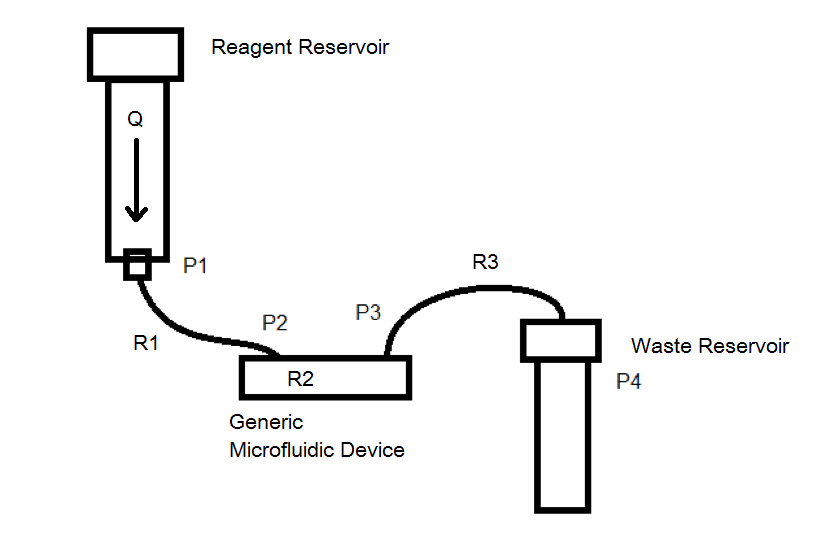
\includegraphics[width=01.0\columnwidth]{resistanceSystem.PNG} 
\caption[Hydraulic Resistance of System]{The microfluidic system detailed from the reagent water column to the waste reservoir.} % The text in the square bracket is the caption for the list of figures while the text in the curly brackets is the figure caption
\label{fig:resistanceSystem} 
\end{figure}

The fluidic resistance present in the reagent reservoirs and tubing leading to the microfluidic device contribute to overall system resistance, and therefore flowrate. However, if the reservoir and tubing widths are substantially larger than the microfluidic device's channels the resistance and therefore contribution to system's pressure loss may be neglected.

For the purpose of quantifying the contribution to total pressure loss of tubing in a generic system the following arbitrary values are applied to first solve for the flowrate at an arbitrary applied pressure of 500mbar. Assume that $P_4$ is equivalent to atmospheric pressure, 0 Pa, and $L_1=L_3= 0.500 \ m$, $L_2=0.010 \ m$, viscosity $n=1 \ cP = 0.001 \ Pa \ s$, tube radius$r=0.00025 \ m$ and channel height $h=0.00005m$. Take $P_1 = 500 \ mbar = 50 \ kPa$ which is mid operational range for the system.

Consider the simple case shown in Figure \vref{fig:resistanceSystem}, and that hydraulic resistances in straight circular and square channels can be approximated as shown in Equations \vref{eq:resCirc} and \vref{eq:resSquare}, respectively.

\begin{equation}
R_1 = R_3 = \frac{8 \eta L}{\pi r^4}= \frac{8 (0.001) (0.500)}{\pi 0.00025^4} = 3.26  \times 10^7 \frac{kg}{m^4s}
\label{eq:resCirc}
\end{equation}

\begin{equation}
R_2 = \frac{28.4 \eta L}{ h^4}= \frac{28.4 (0.001) (0.010)}{ 0.00005^4} = 4.54 \times 10^{13}\frac{kg}{m^4s}
\label{eq:resSquare}
\end{equation}


Clearly the resistance seen over the length of the simplified microfluidic device of dimensions $50 \ um \times 50 \um$ is several orders of magnitude greater than the resistance of the systems input and output tubing. If the total pressure $(P_4 - P_1)$ is assumed to be an arbitrary value of 500mbar, flowrate can be calculated as shown in \vref{eq:resFlow}.

\begin{equation*}
P_4 - P_1 = (R_1 + R_2 + R_3) Q
\end{equation*}

\begin{equation*}
Q = \frac{P_4 - P_1 }{(R_1 + R_2 + R3)}
\end{equation}

\begin{equation}
Q = \frac{50,000}{(2 (3.26*10^7) + 4.54*10^{13})} = 1.10  \times 10^{-9} \frac{m^3}{s} = 1.10  \times 10^{-6} \frac{L}{s}
\label{eq:resFlow}
\end{equation}

Assuming that the system is at steady state and therefore the microfluidic structure (tubing and PDMS) is not expanding due to internal pressure we can infer that by conservation of mass and assumed incompressible fluids that the volumetric flowrate is constant across each of the system pressure points shown in Figure ~\vref{fig:resistanceSystem}. Taking this constant flowrate and the previously found resistances individual pressure drops can be calculated as shown in Equation \vref{eq:resPress}.

\begin{equation*}
P_2 - P_1 = (R_1) Q = 3.59 \times 10^{-2} Pa
\end{equation*}
\begin{equation*}
P_3- P_2 = (R_2)Q = 4.99 \times 10^{4 }Pa
\end{equation*}
\begin{equation}
P_4 - P_3 = (R_3) Q = 3.59 \times 10^{-2} Pa
\label{eq:resPress}
\end{equation}

In this simplified case, representative of a typical microfluidic experimental set-up, the pressure loss due to the tubing as a percentage of the total pressure drop can be calculated as shown in Equation \vref{eq:totalLoss}
\begin{equation}
\frac{P_3-P_2}{P_4-P_1} = \frac{3.59 \times 10^{-2}}{50.00 \times 10^{3}} = 7.18 \times 10^{-7}
\label{eq:totalLoss}
\end{equation}

And so it may be appropriate to neglect the pressure drops across the tubing and assume that the PDFC applied pressure is equivalent to the pressure applied across the microfluidic device. This can be further justified by the fact that the control precision of the system (shown to be 0.25mbar) is larger than the negligible pressure differentials of the tubing sections.

